\chapter{ECM Replay Hardware}


\section{Hardware Requirements}

While a computer connected to a diagnostic link connector can satisfactorily extract ECM data and replay
it to another computer running the diagnostic software, this setup is inconvenient for a number of reasons.
First of all, between the cost of a laptop computer and a diagnostic link connector, this cost of the setup
may reach into the thousands of dollars. Secondly, this equipment may be too cumbersome to carry into the field.
A different solution was required, and the following requirements were arrived at:

\begin{enumerate}
  \item The hardware must be inexpensive.
  \item It must be light and portable.
  \item It must be powerful enough to act as a general computing platform.
  \item It must be capable of communicating using heavy truck network protocols.
\end{enumerate}

\section{Hardware Platform}

\subsection{Computer Hardware}

The replay mechanism hardware is built around a BeagleBone, a commercially available ARM-based miniature computer produced
by Texas Instruments. The most recent iteration of the design, the BeagleBone Black, retails for roughly \$45 and has a 1GHz ARM
processor, 512MB of RAM, and 4GB of onboard flash storage. Weighing just a few ounces, it meets cost-effectiveness and portabilty
requirements.

\begin{figure}[h]
  \centering
  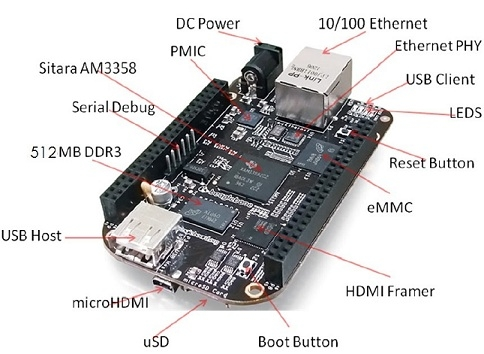
\includegraphics{BeagleBoneBlack}
  \caption{Beaglebone Black}
  \label{fig:BBB}
\end{figure}

\subsection{Capes}

One of the main reasons for adopting the BeagleBone platform is the capability to add functionality using expansion boards, known
as Capes. Commercially available capes include a RS-485 cape and a CAN cape, supporting the physical layers of J1708/J1587 and J1939
with little to no modification.


\begin{figure}[h]
  \centering
  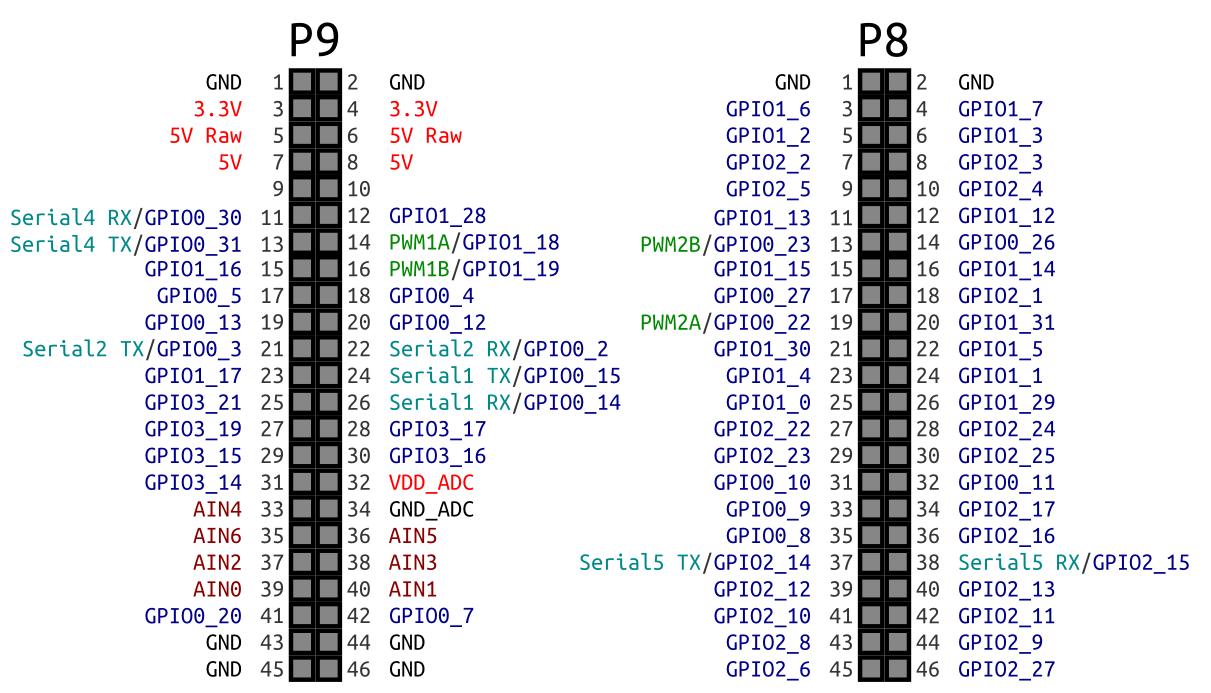
\includegraphics{BeaglebonePinout}
  \caption{Pinout of a Beaglebone Black}
  \label{fig:BBB-pinout}
\end{figure}

\section{Custom Cape}

As the currently available commercial options did not allow for communicating both over J1708 and J1939 networks, a custom
hardware solution was required. A custom cape was designed for heavy vehicle communications. A schematic is included in 
Appendex <include appendix label here>

The J1939 network interface required CAN transceiver hardware. The BeagleBone includes CAN hardware on the board, with access
to the module provided on pins <pins>. Likewise, the J1708/J1587 stack required J1708 hardware. An RS485 transceiver chip from TI
was wired up according to the specifications in the J1708 standard, and accessed through the BeagleBone's UART interface.

\subsection{Drivers}

Driver support for CAN was already well-documented in the BeagleBone; all that was required was to implement the J1939
functionality on top of it. An existing implementation of J1939 for the Linux kernel was found and compiled into
the BeagleBone's kernel as a module. As the remainder of the program was implemented in the Python programming language,
the Python socket module was also patched to work with J1939.

J1708 software drivers for Linux were nonexistent, so new drivers had to be written. Driver code is included in the
appendix.
